\documentclass[12pt]{article}

% Opening
\title{Applied Combinatorics Homework 6}
\author{Akash Narayanan}
\usepackage{amsmath, amsfonts, amssymb, amsthm, enumitem, tikz}
\usepackage{caption, subcaption, float}

% Problem counters
\newcounter{chapternumber}


% Problem environment
\theoremstyle{definition}
\newtheorem{problem-internal}{Problem}[chapternumber]
\newenvironment{problem}{
  \medskip
  \begin{problem-internal}
}{
\end{problem-internal}
}

% Solution environment
\newenvironment{solution}{
  \begin{proof}[Solution]
    \vspace{-8px}
    \setlength{\parskip}{4px}
    \setlength{\parindent}{0px}
}{
\end{proof}
}

\begin{document}

  \maketitle

  % Problem 10.1
  \setcounter{chapternumber}{10}
  \begin{problem}
    Our gang of seven (Alice, Bob, Carlos, Dave, Xing, Yolanda and Zori) are students in a class with a total enrollment of 35. The professor chooses three students at random to go to the board to work challenge problems.
    \begin{enumerate}[label={\alph*.}]
      \item What is the probability that Yolanda is chosen?
      \item What is the probability that Yolanda is chosen and Zori is not?
      \item What is the probability that exactly two members of the club are chosen?
      \item What is the probability that none of the seven members of the club are chosen?
    \end{enumerate}
  \end{problem}

  \begin{solution}
    \hfill
    \begin{enumerate}[label={\alph*.}]
      \item There are a total of \(C(35, 3)\) possible choices,  of which \(C(34, 3)\) do not contain Yolanda. Then the probability is
      \begin{align*}
        P &= \frac{C(35, 3) - C(34, 3)}{C(35, 3)} \\
        &= 1 - \frac{5984}{6545} \\
        &= \frac{3}{35} \approx 0.0857
      \end{align*}

      \item The probability of this occurring is simply the probability that Yolanda is chosen multiplied by the probability that Zori is not chosen. The latter has probability
      \begin{align*}
        \frac{C(34, 3)}{C(35, 3)} = \frac{32}{35}
      \end{align*}
      Then the probability of both events occurring is
      \begin{align*}
        P &= \frac{3}{35} \cdot \frac{32}{35} \\
        &= \frac{96}{1225} \approx 0.0784
      \end{align*}

      \item We consider the possibilities for exactly two members being chosen out of the group of seven. Then the probability is
      \begin{align*}
        P &= \frac{C(7, 2) \cdot C(33 - 5, 1)}{C(35, 3)} \\
        &= \frac{21 \cdot 28}{6545} \\
        &= \frac{84}{935} \approx 0.0898
      \end{align*}

      \item We simply consider the possibilities of the professor choosing members from the 28 students not in the club. Then the probability is
      \begin{align*}
        P &= \frac{C(28, 3)}{C(35, 3)} \\
        &= \frac{468}{935} \approx 0.5005
      \end{align*}
    \end{enumerate}
  \end{solution}


  % Problem 10.2
  \begin{problem}
    Bob says to no one in particular, ``Did you know that the probability that you will get at least one `7' in three rolls of a pair of dice is slightly less than 1/2? On the other hand, the probability that you'll get at least one `5' in six rolls of the dice is just over 1/2." Is Bob on target, or out to lunch?
  \end{problem}

  \begin{solution}
    We consider the Bernoulli trial setup, in which the probability of success (rolling a 7) is \(\frac{1}{6}\) and the probability of failure (not rolling a 7) is \(\frac{5}{6}\). Then given 3 trials, the probability of 1 success is
    \begin{align*}
      P &= 1 - \left(\frac{5}{6}\right)^{3} \\
      &= \frac{91}{216} \approx 0.4213
    \end{align*}
    On the other hand, consider the probability of rolling a 5, which is \(\frac{1}{9}\). This implies the probability of not rolling a 5 is \(\frac{8}{9}\). Then given 6 trials, the probability of rolling a 5 at least once is
    \begin{align*}
      P &= 1 - \left(\frac{8}{9}\right)^{6} \\
      &= \frac{269297}{531441} \approx 0.5067
    \end{align*}
  \end{solution}


  % Problem 10.3
  \begin{problem}
    Consider the spinner shown in the figure below.

    \begin{figure}[H]
      \centering
      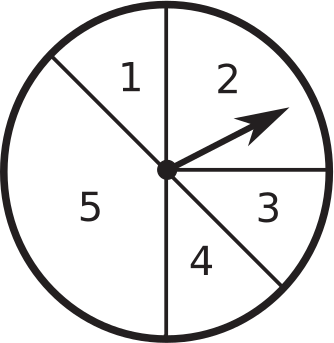
\includegraphics[scale=0.5]{media/spinner.png}
    \end{figure}

    \begin{enumerate}[label={\alph*.}]
      \item What is the probability of getting at least one ``5" in three spins?
      \item What is the probability of getting at least one ``3" in three spins?
      \item If you keep spinning until you get either a ``2" or a ``5", what is the probability that you get a ``2" first?
      \item If you receive \(i\) dollars when the spinner halts in region \(i\), what is the expected value? Since three is right in the middle of the possible outcomes, is it reasonable to pay three dollars to play this game?
    \end{enumerate}
  \end{problem}

  \begin{solution}
    \hfill
    \begin{enumerate}[label={\alph*.}]
      \item The probability of getting a 5 in a single spin looks like \(\frac{3}{8}\). That is, the probability of not spinning a 5 is \(\frac{5}{8}\). Then the probability of spinning at least one 5 in 3 spins is
      \begin{align*}
        P &= 1 - \left(\frac{5}{8}\right)^{3} \\
        &= \frac{387}{512} \approx 0.7559
      \end{align*}

      \item The probability of getting a 3 in a single spin looks like \(\frac{1}{8}\), so the probability of not spinning a 3 is \(\frac{7}{8}\). Then the probability of spinning a 3 in 3 spins is
      \begin{align*}
        P &= 1 - \left(\frac{7}{8}\right)^{3} \\
        &= \frac{169}{512} \approx 0.3301
      \end{align*}

      \item Consider spinning a 2 to be a success, spinning a 5 to be a failure, and spinning anything else to be neutral. The probability of success is \(p_{s} = \frac{1}{4}\), the probability of failure is \(p_{f} = \frac{3}{8}\), and the probability of neutral is \(p_{n} = \frac{3}{8}\). The overall probability of success \(P\) is given by the sum of all independent events that end with \(p_{s}\). That is
      \begin{align*}
        P &= p_{s} + p_{n}p_{s} + p_{n}^{2}p_{s} + p_{n}^{3}p_{s} \cdots \\
        &= p_{s} \sum_{i = 0}^{\infty} p_{n}^{i} = p_{s} \cdot \frac{1}{1 - p_{n}} \\
        &= \frac{1}{4} \cdot \frac{8}{5} = \frac{2}{5}
      \end{align*}

      \item Let \(X\) be a random variable such that \(X(i) = i\). We want to calculate the expected value \(E[X]\). Recall that
      \begin{align*}
        E[X] = \sum_{i \in \Omega} X(i)P(i)
      \end{align*}
      where \(\Omega\) is the underlying set of the probability space. In this case, \(\Omega = \{1, 2, 3, 4, 5\}\). Then we have
      \begin{align*}
        E[X] &= 1 \cdot \frac{1}{8} + 2 \cdot \frac{1}{4} + 3 \cdot \frac{1}{8} + 4 \cdot \frac{1}{8} + 5 \cdot \frac{3}{8} \\
        &= \frac{27}{8} = 3.375
      \end{align*}
      That is, one can expect to win \$3.375 from playing the game. Paying \$3 is reasonable because one expects to earn an average of \$0.375 per game, and they can make a profit.
    \end{enumerate}
  \end{solution}

  % Problem 10.4
  \begin{problem}
    Alice proposes to Bob the following game. Bob pays one dollar to play.
    Fifty balls marked \(1, 2, \ldots 50\) are placed in a big jar, stirred around, and then drawn out one by one by Zori, who is wearing a blindfold.
    The result is a random permutation \(\sigma\) of the integers \(1, 2, \ldots, 50\).
    Bob wins with a payout of two dollars and fifty cents if the permutation \(\sigma\) is a derangement, i.e., \(\sigma(i) \neq i\) for all \(i = 1, 2, \ldots, n\).
    Is this a fair game for Bob? If not, how should the payoff be adjusted to make it fair?
  \end{problem}

  \begin{solution}
    Using Inclusion-Exclusion, we have the number of derangements \(d_{n}\) on a set with \(n\) elements is
    \begin{align*}
      d_{n} = \sum_{k=0}^{n} (-1)^{k} {n \choose k} (n-k)!
    \end{align*}
    while the number of permutations on a set with \(n\) elements is \(n!\). Of course, when \(n=50\) these numbers grow tiresomely large. However, we can apply a fact derived in class:
    \begin{equation*}
      \lim_{n \to \infty} \frac{d_{n}}{n!} = \frac{1}{e}
    \end{equation*}
    We can use this value to approximate the probability of a random permutation being a derangement. Given this, it is evident that the game is not fair. As it exists, the expected value of the game is
    \begin{align*}
      E[X] &= (-1) (1) + (2.50) \frac{1}{e} \\
           &\approx -0.08
    \end{align*}
    That is, the game is unfair for Bob, who needs the permutation to be a derangement. The payoff should be adjusted to be close to \(e\) if Bob wins. This ensures that the expected value is
    \begin{align*}
      E[X] &= (-1) (1) + (e) \frac{1}{e} \\
           &= 0
    \end{align*}
    Since the expected value is 0, the game is fair and no net profit or loss is to be expected.
  \end{solution}

  % Problem 13.2
  \setcounter{chapternumber}{13}
  \setcounter{problem-internal}{1}
  \begin{problem}
    Alice claims to have found a (valid) network flow of value 20 in the network shown below. Bob tells her that there's no way she's right, since no flow has value greater than 18. Who's right and why?

    \begin{figure}[H]
      \centering
      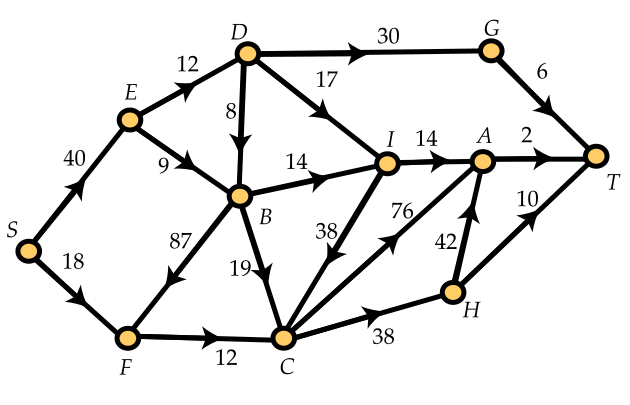
\includegraphics[scale=0.5]{media/network.png}
    \end{figure}

  \end{problem}

  \begin{solution}
    Bob is correct. Recall that the value of a flow can never exceed the capacity of a cut. Consider the cut in which one vertex set contains only \(T\). Then the capacity of the cut is the sum of the capacities of the edges leading into \(T\), which is \(6 + 2 + 10 = 18\). Thus, the capacity of the cut is 18 so no flow can exceed a value of 18.
  \end{solution}

  % Problem 13.3
  \begin{problem}
    Find an augmenting path \(P\) with \textit{at least one backward edge} for the flow \(\phi\) in the network shown below. What is the value of \(\delta\) for \(P\)? Carry out an update of \(\phi\) using \(P\) to obtain a new flow \(\hat{\phi}\). What is the value of \(\hat{\phi}\)?

    \begin{figure}[H]
      \centering
      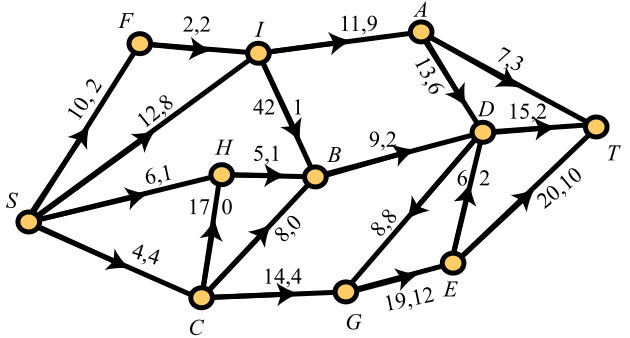
\includegraphics[scale=0.5]{media/aug_path.png}
    \end{figure}

  \end{problem}

  \begin{solution}
    Consider the augmenting path \(P = (S, H, B, D, A, T)\). The edge \((D, A)\) is backwards. For this path, we have \(\delta_{1} = \min \{5, 4, 7, 4\} = 4\) and \(\delta_{2} = \min \{4\} = 4\). Then \(\delta = \min \{\delta_{1}, \delta_{2}\} = 4\). The updated flow \(\hat{\phi}\) has the same flow on all edges except for the following:

    \begin{center}
      \begin{tabular}{c c}
        Edge & New Flow \\
        \((S, H)\) & 6, 5 \\
        \((H, B)\) & 5, 5 \\
        \((B, D)\) & 9, 6 \\
        \((D, A)\) & 13, 2 \\
        \((A, T)\) & 7, 7
      \end{tabular}
    \end{center}

    The value of \(\hat{\phi}\) is \(20 + 15 + 7 = 42\).
  \end{solution}

  % Problem 13.6
  \setcounter{problem-internal}{5}
  \begin{problem}
    Find the capacity of the cut \((L, U)\) with
    \begin{align*}
      L = \{S, F, D, B, A\} && \text{and} && U = \{H, C, I, G, E, T\}
    \end{align*}
    in the network shown below.

    \begin{figure}[H]
      \centering
      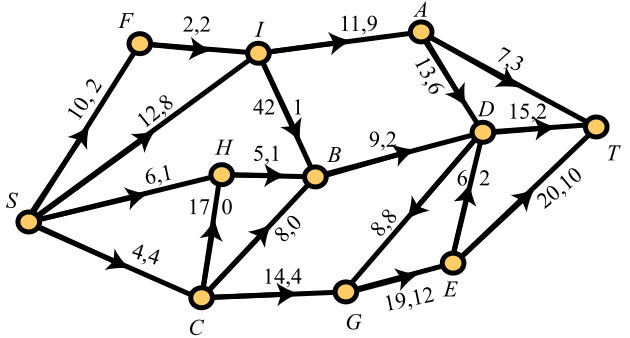
\includegraphics[scale=0.5]{media/aug_path.png}
    \end{figure}

  \end{problem}

  \begin{solution}
    The capacity of the cut is the sum of the capacity of each forward edge from \(L\) to \(U\). All such edges and their capacities are listed below:

    \begin{center}
      \begin{tabular}{c c}
        Forward Edge & Capacity \\
        \((S, I)\) & 12 \\
        \((S, H)\) &  6 \\
        \((S, C)\) &  4 \\
        \((F, I)\) &  2 \\
        \((D, G)\) &  8 \\
        \((D, T)\) & 15 \\
        \((A, T)\) &  7
      \end{tabular}
    \end{center}

    Then the capacity of the cut is \(12 + 6 + 4 + 2 + 8 + 15 + 7 = 54\).
  \end{solution}
\end{document}
